\documentclass{article}
\usepackage[utf8]{inputenc}
\usepackage{graphicx} % Required for the inclusion of images
\graphicspath{{images/}}




%----------------------------------------------------------------------------------------
%	DOCUMENT INFORMATION
%----------------------------------------------------------------------------------------

\title{Music Playlist [Pure Html]} % Title
\author{Lorenzo Campana} % Author name
\date{\today}

\begin{document}
\maketitle 
\begin{center}
\begin{tabular}{l r}
Matricola: & 907081\\ % Partner names
Codice Persona: & 10605775\\
Docente: & Piero Fraternali
\end{tabular}
\end{center}


\section{Requirements}
Un’applicazione web consente la gestione di una playlist di brani musicali. Playlist e brani sono personali di ogni utente e non condivisi. Ogni brano musicale è memorizzato nella base di dati mediante un titolo , l‘immagine e il titolo dell’album da cui il brano è tratto, il nome dell’interprete (singolo o gruppo) dell’album,  l’anno di pubblicazione dell’album, il genere musicale (si supponga che i generi siano prefissati) e il file musicale. L’utente, previo login, può creare brani mediante il caricamento dei dati relativi e raggrupparli in playlist.  Una playlist è un insieme di brani scelti tra quelli caricati dallo stesso utente ordinati per data decrescente dall’anno di pubblicazione dell’album. Una playlist ha un titolo e una data di creazione ed è associata al suo creatore.  A seguito del login, l’utente accede all’HOME PAGE che presenta l’elenco delle proprie playlist, ordinate per data di creazione decrescente, una form per caricare un brano con tutti i dati relativi e una form per creare una nuova playlist inizialmente vuota. Quando l’utente clicca su una playlist nell’HOME PAGE, appare la pagina PLAYLIST PAGE che contiene inizialmente una tabella di una riga e cinque colonne. Ogni cella contiene  il titolo di un brano e l’immagine dell’album da cui proviene. Se la playlist è inizialmente vuota compare un messaggio: “La playlist non contiene ancora brani musicali”. I brani sono ordinati da sinistra a destra per data decrescente dell’album di pubblicazione. Se la playlist contiene più di cinque brani, sono disponibili comandi per vedere il precedente e successivo gruppo di brani. Se la pagina PLAYLIST mostra il primo gruppo e ne esistono altri successivi nell’ordinamento, compare a destra della riga il bottone SUCCESSIVI, che permette di vedere il gruppo successivo. Se la pagina PLAYLIST mostra l’ultimo gruppo e ne esistono altri precedenti nell’ordinamento, compare a sinistra della riga il bottone PRECEDENTI, che permette di vedere i cinque brani precedenti. Se la pagina PLAYLIST mostra un blocco e esistono sia precedenti sia successivi, compare a destra della riga il bottone SUCCESSIVI e a sinistra il bottone PRECEDENTI. La pagina PLAYLIST contiene anche una form che consente di selezionare e  aggiungere un brano alla playlist corrente. A seguito dell’aggiunta di un brano alla playlist corrente, l’applicazione visualizza nuovamente la pagina  a partire dal primo blocco della playlist. Quando l’utente seleziona il titolo di un brano, la pagina PLAYER mostra tutti i dati del brano scelto e il player audio per la riproduzione del brano.
 
\section{Database design}

\subsection{ER diagram}
\begin{figure}[h]
\centering
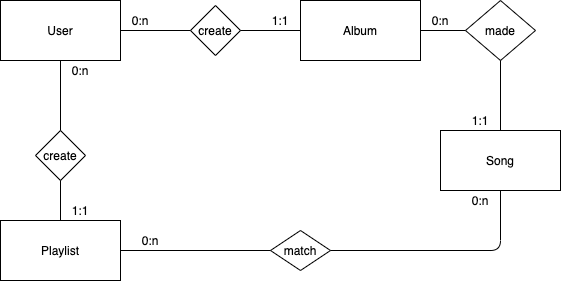
\includegraphics[width=1\textwidth]{ERdiagram}
\caption{ER diagram}
\label{fig:ERdiagram}
\end{figure}

\newpage

\subsection{Database model}
\begin{figure}[h]
\centering
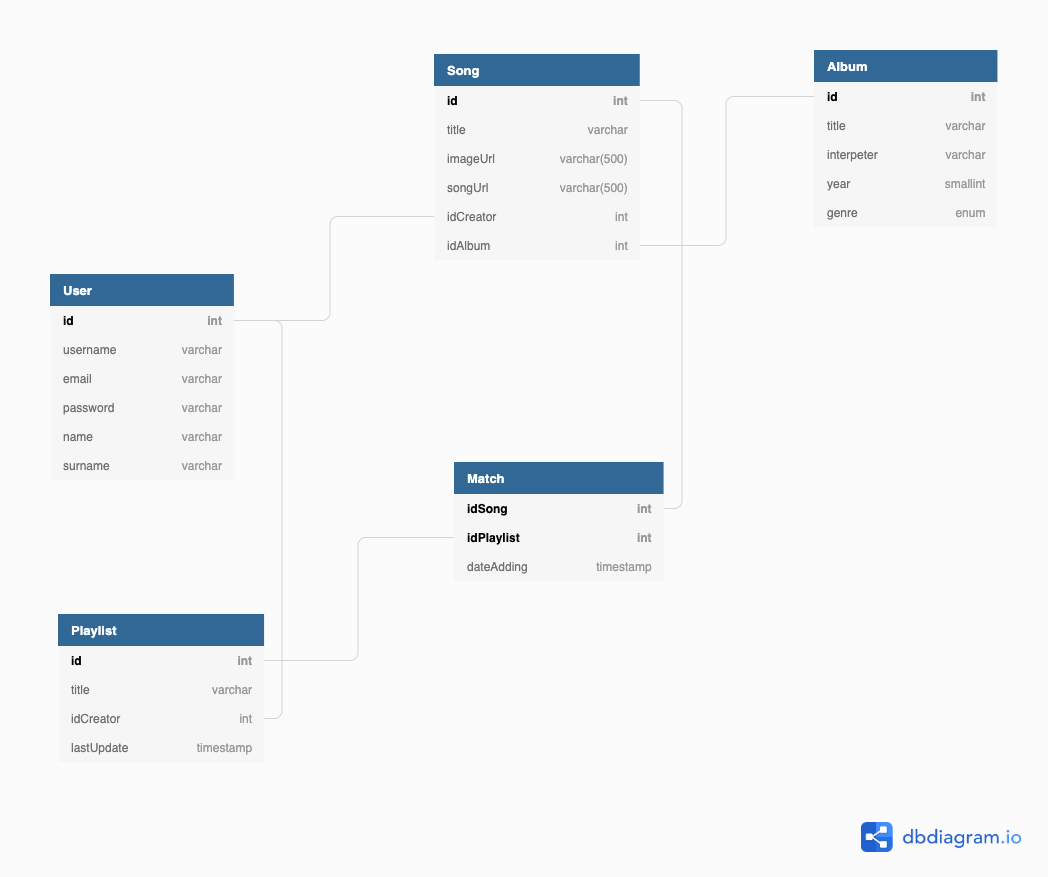
\includegraphics[width=1\textwidth]{databaseProject}
\caption{database model}
\label{fig:databaseProject}
\end{figure}
\newpage


\section{Application Design}

\subsection{Components}

\begin{itemize}
    \item Model objects (Beans)
    \texttt{
    \begin{itemize}
        \item User
        \item Genre
        \item Match
        \item Playlist
        \item Song
    \end{itemize}
    }
    \item Data Access Objects (Classes)
    \begin{itemize}
        \item AlbumDAO
        \begin{itemize}
            \item \texttt{int createAlbum(Album album)}
            \item \texttt{int findAlbumId(Album album)}
            \item \texttt{Album findAlbumById(int albumId)}
            \item \texttt{ArrayList<Album> findAllUserAlbumsById(int userId)} 
        \end{itemize}
        \item UserDAO
        \begin{itemize}
            \item \texttt{int createUser(User user)}
            \item \texttt{User findUserById(int idUser)}
            \item \texttt{int findIdOfUserByEmail(String email)}
            \item \texttt{boolean isPasswordCorrect(int idUser, String password)}
        \end{itemize}
        \item SongDAO
        \begin{itemize}
            \item \texttt{int createSong(Song song)}
            \item \texttt{int findSongId(Song song)}
            \item \texttt{Song findSongById(int songId)}
            \item \texttt{ArrayList<Song> findAllSongByUserId(int userId)}
        \end{itemize}
        \item PlaylistDAO
        \begin{itemize}
            \item \texttt{int createPlaylist(String title, int idCreator)}
            \item \texttt{ArrayList<Playlist> findAllPlaylistByUserId(int userId)}
            \item \texttt{Playlist findPlaylistById(int playlistId)}
        \end{itemize}
        \item MatchDAO
        \begin{itemize}
            \item \texttt{int createMatch(Match match)}
            \item \texttt{ArrayList <Integer> findAllSongIdOfPlaylist(int idPlaylist, int userId)}
        \end{itemize}
    \end{itemize}
    \item Controllers (Servlets)
    \texttt{
    \begin{itemize}
        \item AddSongToPlaylist
        \item CreateAlbum
        \item CreatePlaylist
        \item CreateSong
        \item GetHomePage
        \item GetPlayer
        \item GetPlaylist
        \item ShowFile
        \item SubmitLogin
        \item SubmitRegistration
        \item Logout
    \end{itemize}
    }
    \item Views (Templates)
    \texttt{
    \begin{itemize}
        \item ErrorPage.html
        \item HomePage.html
        \item Login.html
        \item Player.html
        \item PlaylistPage.html
        \item Register.html
    \end{itemize}
    }
\end{itemize}

\subsection{IFML}
\begin{figure}[h]
\centering
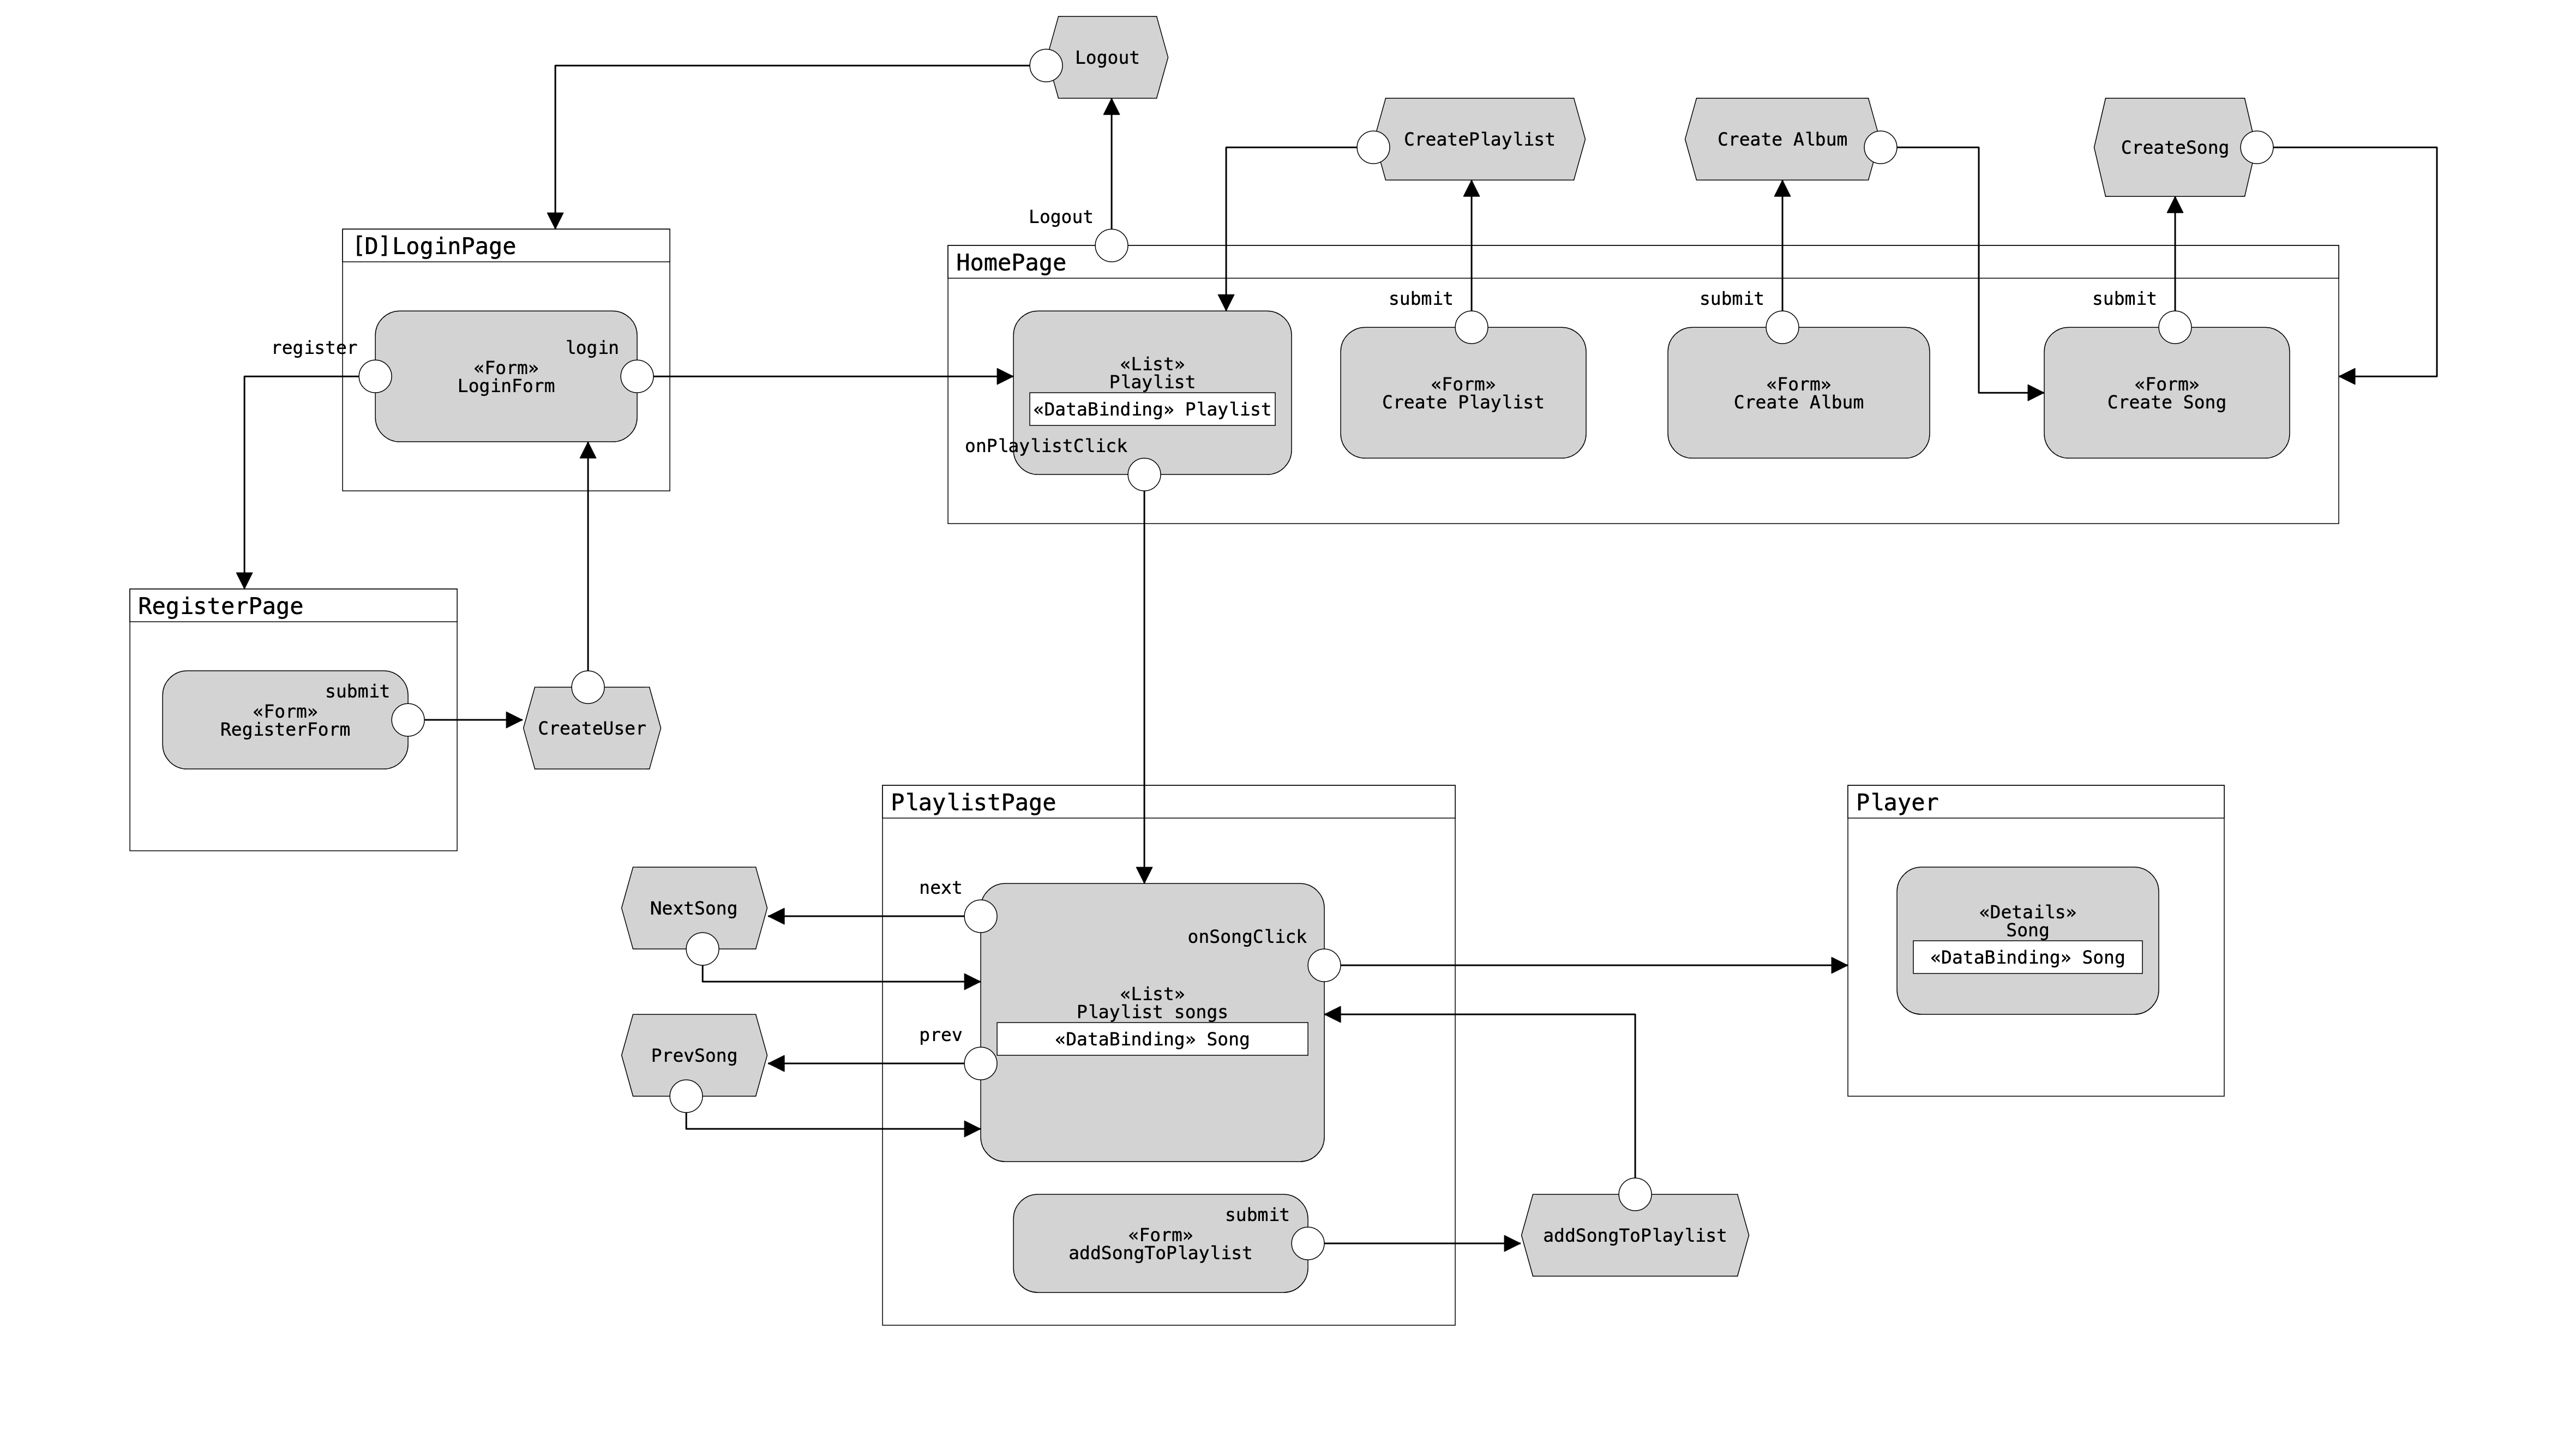
\includegraphics[width=1\textwidth]{model}
\caption{Ifml model}
\label{fig:model}
\end{figure}



%---------------------------SEQUENCE DIAGRAM SECTION
\newpage
\section{Event sequence diagram}

\subsection{Forward method}
To simplify the sequence diagram below, each servlet uses the method
\texttt{forward(HttpServletRequest request, HttpServletResponse response, String path)} that is responsible to take the WebContext and process the TemplateEngine as shown below

\begin{figure}[h]
\centering
\includegraphics[width=1\textwidth]{sequenceDiagram/forward(METHOD).png}
\caption{forward method}
\label{fig:ForwardMethod}
\end{figure}

\newpage
\subsection{Login}
\begin{figure}[h]
\centering
\includegraphics[width=1\textwidth]{sequenceDiagram/SubmitLogin(POST).png}
\caption{POST /SubmitLogin}
\label{fig:SubmitLogin}
\end{figure}

\newpage
\subsection{Registration}
\begin{figure}[h]
\centering
\includegraphics[width=1\textwidth]{sequenceDiagram/SubmitRegistration(POST).png}
\caption{POST /SubmitRegistration}
\label{fig:SubmitRegistration}
\end{figure}

\newpage
\subsection{Logout}
\begin{figure}[h]
\centering
\includegraphics[width=1\textwidth]{sequenceDiagram/Logout(POST).png}
\caption{POST /Logout}
\label{fig:Logout}
\end{figure}

\newpage
\subsection{Home Page}
\begin{figure}[h]
\centering
\includegraphics[width=1\textwidth]{sequenceDiagram/GetHomePage(GET).png}
\caption{GET /GetHomePage}
\label{fig:GetHomePage}
\end{figure}


\newpage
\subsubsection{Playlist creation}
\begin{figure}[h]
\centering
\includegraphics[width=1\textwidth]{sequenceDiagram/CreatePlaylist(POST).png}
\caption{POST /CreatePlaylist}
\label{fig:CreatePlaylist}
\end{figure}

\newpage
\subsubsection{Song creation}
\begin{figure}[h]
\centering
\includegraphics[width=1\textwidth]{sequenceDiagram/CreateSong(POST).png}
\caption{POST /CreateSong}
\label{fig:CreateSong}
\end{figure}

\newpage
\subsubsection{Album creation}
\begin{figure}[h]
\centering
\includegraphics[width=1\textwidth]{sequenceDiagram/CreateAlbum(POST).png}
\caption{POST /CreateAlbum}
\label{fig:CreateAlbum}
\end{figure}

\newpage
\subsection{Playlist Page}
\begin{figure}[h]
\centering
\includegraphics[width=0.9\textwidth]{sequenceDiagram/GetPlaylist(GET).png}
\caption{GET /GetPlaylist}
\label{fig:GetPlaylist}
\end{figure}


\newpage
\subsubsection{Add song to playlist}
\begin{figure}[h]
\centering
\includegraphics[width=1\textwidth]{sequenceDiagram/AddSongToPlaylist(POST).png}
\caption{POST /AddSongToPlaylist}
\label{fig:AddSongToPlaylist}
\end{figure}


\newpage
\subsection{Player Page}
\begin{figure}[h]
\centering
\includegraphics[width=1\textwidth]{sequenceDiagram/GetPlayer(GET).png}
\caption{GET /GetPlayer}
\label{fig:GetPlayer}
\end{figure}





\end{document}
